%% ============================================================
%%  Quantum Boltzmann Machines
%%  From Quantum Neural Networks to Quantum Generative Models
%%  Author: Morten Hjorth-Jensen
%%  Department of Physics, University of Oslo
%% ============================================================
\documentclass[aspectratio=169,10pt]{beamer}

%% ── Theme & colours ─────────────────────────────────────────────
\usetheme{Madrid}
\usecolortheme{seahorse}
\usefonttheme[onlymath]{serif}

\setbeamercolor{frametitle}{bg=blue!15!white,fg=blue!60!black}
\setbeamercolor{title}{fg=blue!70!black}
\setbeamercolor{block title}{bg=blue!20!white,fg=blue!60!black}
\setbeamercolor{block body}{bg=blue!5!white}
\setbeamercolor{alerted text}{fg=red!60!black}
\setbeamertemplate{navigation symbols}{}
\setbeamertemplate{footline}{%
  \leavevmode\hbox{%
    \begin{beamercolorbox}[wd=.25\paperwidth,ht=2.25ex,dp=1ex,center]{author in head/foot}%
      \usebeamerfont{author in head/foot}\insertshortauthor
    \end{beamercolorbox}%
    \begin{beamercolorbox}[wd=.50\paperwidth,ht=2.25ex,dp=1ex,center]{title in head/foot}%
      \usebeamerfont{title in head/foot}\insertshorttitle
    \end{beamercolorbox}%
    \begin{beamercolorbox}[wd=.25\paperwidth,ht=2.25ex,dp=1ex,right]{date in head/foot}%
      \usebeamerfont{date in head/foot}\insertshortdate{}\hspace*{1em}%
      \insertframenumber{}/\inserttotalframenumber\hspace*{1ex}
    \end{beamercolorbox}}%
  \vskip0pt}

%% ── Packages ────────────────────────────────────────────────────
\usepackage{amsmath,amssymb,bm,physics}
\usepackage{braket}
\usepackage{graphicx}
\usepackage{booktabs}
\usepackage{xcolor}
\usepackage{tikz}
\usetikzlibrary{positioning,arrows.meta,shapes.geometric,fit,decorations.pathreplacing}
\usepackage{quantikz}
\usepackage{listings}
\usepackage{hyperref}

%% ── Python listing style ─────────────────────────────────────────
\lstset{
  language=Python,
  basicstyle=\ttfamily\scriptsize,
  keywordstyle=\color{blue!70!black}\bfseries,
  commentstyle=\color{gray},
  stringstyle=\color{red!60!black},
  breaklines=true,
  frame=single,
  backgroundcolor=\color{blue!3!white},
  xleftmargin=4pt, xrightmargin=4pt
}

%% ── Convenience macros ──────────────────────────────────────────
\newcommand{\KL}[2]{D_{\mathrm{KL}}\!\left(#1\,\|\,#2\right)}
\newcommand{\Hilbert}{\mathcal{H}}
%% \week used in the course-summary section
\newcommand{\week}[1]{\textcolor{blue!60!black}{\textbf{#1}}}
%% colour alias used in the perspectives divider
\colorlet{qblue}{blue!50!black}

%% ── Metadata ────────────────────────────────────────────────────
\title[Quantum Boltzmann Machines]{Quantum Boltzmann Machines and Summary of Course}
%\subtitle{From Quantum Neural Networks to Quantum Generative Models}
\author[M.~Hjorth-Jensen]{Morten Hjorth-Jensen}
\institute[UiO]{Department of Physics \& CCSE\\University of Oslo}
\date{May 20, 2026}

%% ============================================================
\begin{document}
%% ============================================================

\begin{frame}
  \titlepage
\end{frame}

\begin{frame}{Outline}
  \tableofcontents[hidesubsections]
\end{frame}

%% ============================================================
\section{Classical Boltzmann Machines}
%% ============================================================


\begin{frame}{From Discriminative to Generative Models}
  \begin{columns}[T]
    \column{0.52\textwidth}
      \begin{block}{Discriminative QNN (what we had)}
        \begin{itemize}\itemsep1pt
          \item Input $x$ encoded via $U(x)$
          \item Output: class label or regression value
          \item Minimise: $\mathcal{L} = \sum_k (f(x_k)-y_k)^2$
          \item Goal: learn $p(y|x)$
        \end{itemize}
      \end{block}
      \vspace{0.15cm}
      \begin{alertblock}{Generative QML (our goal now)}
        \begin{itemize}\itemsep1pt
          \item \textbf{No} input encoding needed
          \item Output: full probability distribution $p(x)$
          \item Minimise: $\KL{p_{\rm data}}{p_\theta}$
          \item Goal: learn to \emph{sample} from $p_{\rm data}$
        \end{itemize}
      \end{alertblock}
    \column{0.44\textwidth}
      \textbf{Generative models in QML:}
      \begin{itemize}\itemsep2pt
        \item Quantum Boltzmann Machines (QBM) — \emph{this talk}
        \item Quantum Circuit Born Machines (QCBM)
        \item Quantum GANs
        \item Quantum Variational Autoencoders
      \end{itemize}
      \vspace{0.2cm}
      \textbf{Key difference:}\\
      QBMs model distributions via a \emph{thermal state}
      (density matrix) rather than a pure variational state.
  \end{columns}
\end{frame}




\begin{frame}{Classical Restricted Boltzmann Machine}
  \begin{columns}[T]
    \column{0.52\textwidth}
      An RBM has \textbf{visible} units $\mathbf{v}\in\{0,1\}^n$
      and \textbf{hidden} units $\mathbf{h}\in\{0,1\}^m$.

      \textbf{Energy function:}
      \[
        E(\mathbf{v},\mathbf{h}) =
        -\sum_i a_i v_i
        -\sum_j b_j h_j
        -\sum_{ij} v_i W_{ij} h_j
      \]
      \textbf{Joint distribution and partition function:}
      \[
        p(\mathbf{v},\mathbf{h}) = \frac{e^{-\beta E}}{Z},\quad
        Z = \sum_{\mathbf{v},\mathbf{h}} e^{-\beta E}
      \]
      \textbf{Marginal over visible:}
      \[
        p(\mathbf{v}) = \frac{1}{Z}\sum_\mathbf{h} e^{-\beta E(\mathbf{v},\mathbf{h})}
      \]
    \column{0.44\textwidth}
      \vspace{0.1cm}
      \begin{center}
      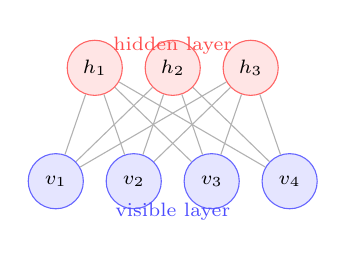
\begin{tikzpicture}[scale=0.9,
        vis/.style={circle,draw=blue!60,fill=blue!10,minimum size=0.7cm,
                    font=\scriptsize},
        hid/.style={circle,draw=red!60,fill=red!10,minimum size=0.7cm,
                    font=\scriptsize}]
        \foreach \i/\lbl in {1/$v_1$,2/$v_2$,3/$v_3$,4/$v_4$}{
          \node[vis] (v\i) at (\i*1.1-0.55,0) {\lbl};
        }
        \foreach \j/\lbl in {1/$h_1$,2/$h_2$,3/$h_3$}{
          \node[hid] (h\j) at (\j*1.1+0.0,1.6) {\lbl};
        }
        \foreach \i in {1,...,4}
          \foreach \j in {1,...,3}
            \draw[gray!60,thin] (v\i)--(h\j);
        \node[below=0.15cm,font=\scriptsize,blue!70] at (2.2,0)
          {visible layer};
        \node[above=0.05cm,font=\scriptsize,red!70] at (2.2,1.6)
          {hidden layer};
      \end{tikzpicture}
      \end{center}
      \vspace{0.1cm}
      No intra-layer connections $\Rightarrow$ tractable
      conditional independence:
      \[
        p(h_j=1|\mathbf{v}) = \sigma\!\bigl(b_j+\sum_i W_{ij}v_i\bigr)
      \]
  \end{columns}
\end{frame}

\begin{frame}{RBM Training: Contrastive Divergence}
  \begin{columns}[T]
    \column{0.52\textwidth}
      \textbf{Log-likelihood gradient:}
      \[
        \frac{\partial\ln p(\mathbf{v})}{\partial W_{ij}}
        = \langle v_i h_j\rangle_{\rm data}
        - \langle v_i h_j\rangle_{\rm model}
      \]
      \begin{itemize}
        \item Data term: easy (one forward pass)
        \item Model term: hard (requires summing over
              all $\mathbf{v},\mathbf{h}$)
      \end{itemize}

      \textbf{Contrastive Divergence (CD-$k$):}
      \begin{enumerate}
        \item Clamp $\mathbf{v}^{(0)} = \mathbf{v}_{\rm data}$
        \item Run $k$ steps of Gibbs sampling
              $\mathbf{v}^{(0)}\to\mathbf{h}^{(0)}\to
               \mathbf{v}^{(1)}\to\cdots\to\mathbf{v}^{(k)}$
        \item Approximate model term with $\mathbf{v}^{(k)}$
      \end{enumerate}
    \column{0.44\textwidth}
      \begin{block}{CD-$k$ update rule}
        \[
          \Delta W_{ij} \propto
          \langle v_i h_j\rangle_{\rm data}
          - \langle v_i h_j\rangle_k
        \]
        Similarly for biases $a_i$, $b_j$.
      \end{block}
      \vspace{0.3cm}
      \begin{alertblock}{Key limitation}
        The partition function $Z$ is intractable for large
        systems — gradient estimates are biased.
        Quantum hardware promises an exact, unbiased estimate
        of $\langle v_i h_j\rangle_{\rm model}$ via
        \emph{quantum sampling}.
      \end{alertblock}
  \end{columns}
\end{frame}

%% ============================================================
\section{Quantum Boltzmann Machines: Definition and Structure}
%% ============================================================

\begin{frame}{From Classical to Quantum Gibbs States}
  \begin{columns}[T]
    \column{0.52\textwidth}
      Replace binary units with \textbf{qubits} and the
      classical energy function with a \textbf{quantum Hamiltonian}:

      \medskip
      \textbf{Classical:} $p(\mathbf{v}) = e^{-\beta E(\mathbf{v})}/Z$

      \medskip
      \textbf{Quantum:} The thermal (Gibbs) state
      \[
        \boxed{
          \rho(\theta) = \frac{e^{-\beta H(\theta)}}{\Tr[e^{-\beta H(\theta)}]}
        }
      \]
      where $H(\theta)$ is a parametrised quantum Hamiltonian.

      \medskip
      The partition function is now a \emph{quantum trace}:
      \[
        Z(\theta) = \Tr\!\left[e^{-\beta H(\theta)}\right]
        = \sum_k e^{-\beta\epsilon_k(\theta)}
      \]
      where $\{\epsilon_k\}$ are eigenvalues of $H(\theta)$.
    \column{0.44\textwidth}
      \begin{block}{Degrees of freedom}
        \begin{tabular}{ll}
          \toprule
          Classical RBM & QBM \\
          \midrule
          Binary spins $\{0,1\}^n$ & $n$ qubits \\
          Energy $E(\mathbf{v},\mathbf{h})$ & Hamiltonian $H(\theta)$ \\
          Gibbs dist.\ $e^{-\beta E}/Z$ & Gibbs state $e^{-\beta H}/Z$ \\
          Marginal $p(\mathbf{v})$ & Reduced state $\rho_v$ \\
          \bottomrule
        \end{tabular}
      \end{block}
      \vspace{0.2cm}
      \begin{alertblock}{Key gain}
        Quantum off-diagonal (transverse) terms in $H(\theta)$
        allow the QBM to represent \emph{quantum correlations}
        and \emph{superpositions} — beyond any classical BM.
      \end{alertblock}
  \end{columns}
\end{frame}

\begin{frame}{The QBM Hamiltonian}
  \begin{columns}[T]
    \column{0.52\textwidth}
      The most general parametrised $n$-qubit QBM Hamiltonian:
      \[
        H(\theta) = -\sum_i \theta_i^x X_i
                    -\sum_i \theta_i^z Z_i
                    -\sum_{i<j} \theta_{ij}^{zz} Z_i Z_j
                    - \cdots
      \]
      \begin{itemize}
        \item $\theta_i^z$: \textbf{longitudinal fields} (diagonal)
              — classical bias terms, analogous to $a_i$
        \item $\theta_{ij}^{zz}$: \textbf{ZZ couplings} (diagonal)
              — classical two-body interactions, analogous to $W_{ij}$
        \item $\theta_i^x$: \textbf{transverse fields}
              (off-diagonal) — \alert{purely quantum} term,
              no classical analogue
      \end{itemize}
    \column{0.44\textwidth}
      \begin{block}{Thermal state in the eigenbasis}
        \[
          H(\theta)\ket{\epsilon_k} = \epsilon_k\ket{\epsilon_k}
        \]
        \[
          \rho(\theta) = \sum_k
            \frac{e^{-\beta\epsilon_k}}{Z}\ket{\epsilon_k}\bra{\epsilon_k}
        \]
      \end{block}
      \vspace{0.2cm}
      \begin{block}{Classical limit}
        Setting $\theta_i^x = 0$ for all $i$ recovers a classical
        BM: $[H,Z_i]=0$ $\forall i$, so $\rho$ is diagonal in
        the $Z$-basis and reduces to a classical Boltzmann
        distribution.
      \end{block}
  \end{columns}
\end{frame}

\begin{frame}{Visible, Hidden, and Auxiliary Qubits}
  \begin{columns}[T]
    \column{0.52\textwidth}
      Following the classical RBM structure, the $n$ qubits are
      partitioned into:
      \[
        \mathcal{H} = \mathcal{H}_v \otimes \mathcal{H}_h,
        \quad n_v + n_h = n
      \]
      \begin{itemize}
        \item \textbf{Visible} qubits $v$: coupled to the data;
              we observe their reduced state $\rho_v = \Tr_h[\rho]$
        \item \textbf{Hidden} qubits $h$: latent variables
              that are traced out
      \end{itemize}
      The visible marginal is the model distribution:
      \[
        p_\theta(\mathbf{v}) = \bra{\mathbf{v}}\rho_v(\theta)\ket{\mathbf{v}}
      \]
      where $\rho_v(\theta) = \Tr_h\!\left[\frac{e^{-\beta H(\theta)}}{Z}\right]$.
    \column{0.44\textwidth}
      \vspace{0.3cm}
      \begin{center}
      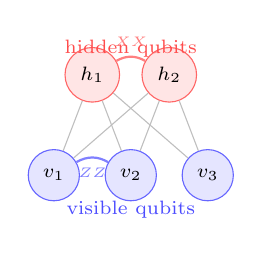
\begin{tikzpicture}[scale=0.85,
        vis/.style={circle,draw=blue!60,fill=blue!10,minimum size=0.65cm,
                    font=\scriptsize},
        hid/.style={circle,draw=red!60,fill=red!10,minimum size=0.65cm,
                    font=\scriptsize}]
        \foreach \i/\lbl in {1/$v_1$,2/$v_2$,3/$v_3$}{
          \node[vis] (v\i) at (\i*1.15,0) {\lbl};
        }
        \foreach \j/\lbl in {1/$h_1$,2/$h_2$}{
          \node[hid] (h\j) at (\j*1.15+0.575,1.5) {\lbl};
        }
        \foreach \i in {1,2,3}
          \foreach \j in {1,2}
            \draw[gray!50,thin] (v\i)--(h\j);
        \draw[blue!50,thick] (v1) to[bend left=30] node[below,font=\tiny]{$ZZ$} (v2);
        \draw[red!50,thick]  (h1) to[bend left=30] node[above,font=\tiny]{$XX$} (h2);
        \node[below=0.2cm,font=\scriptsize,blue!70] at (2.3,0) {visible qubits};
        \node[above=0.1cm,font=\scriptsize,red!70]  at (2.3,1.5) {hidden qubits};
      \end{tikzpicture}
      \end{center}
      \vspace{0.15cm}
      {\small Quantum connections can include $XX$, $YY$, $ZZ$
       within visible, within hidden, and across layers.}
  \end{columns}
\end{frame}

%% ============================================================
\section{Training Quantum Boltzmann Machines}
%% ============================================================

\begin{frame}{The QBM Training Objective}
  \begin{columns}[T]
    \column{0.52\textwidth}
      Given empirical distribution $\pi(\mathbf{v})$, minimise
      the KL divergence $\mathcal{L}(\theta)=\KL{\pi}{p_\theta}$:
      \[
        \mathcal{L}(\theta)
        = \sum_\mathbf{v}\pi(\mathbf{v})\ln\frac{\pi(\mathbf{v})}{p_\theta(\mathbf{v})}
      \]
      Expanding with $p_\theta(\mathbf{v})=\bra{\mathbf{v}}\rho_v\ket{\mathbf{v}}$
      and $\sigma_{\rm data}=\sum_\mathbf{v}\pi(\mathbf{v})\ket{\mathbf{v}}\bra{\mathbf{v}}$:
      \[
        \mathcal{L}(\theta)
        = -\Tr[\sigma_{\rm data}\ln\rho_v(\theta)] + \mathrm{const}
      \]
    \column{0.44\textwidth}
      \begin{alertblock}{Quantum relative entropy}
        The objective equals the quantum relative entropy:
        \[
          \mathcal{L} = S(\sigma_{\rm data}\,\|\,\rho_v(\theta))
        \]
        \[
          = \Tr[\sigma_{\rm data}(\ln\sigma_{\rm data} - \ln\rho_v)]
        \]
        Reduces to classical KL when both states are diagonal.
      \end{alertblock}
      \vspace{0.1cm}
      \begin{block}{Full QBM objective}
        For a quantum target state, use the total quantum
        relative entropy:
        $\mathcal{L} = S(\rho_{\rm target}\,\|\,\rho(\theta))$.
      \end{block}
  \end{columns}
\end{frame}

\begin{frame}{Gradient of the Log-Likelihood}
  \begin{columns}[T]
    \column{0.55\textwidth}
      The gradient of the NLL w.r.t.\ $\theta_\mu$, where
      $H(\theta)=\sum_\mu\theta_\mu\Lambda_\mu$:
      \[
        \frac{\partial\mathcal{L}}{\partial\theta_\mu}
        = \langle\Lambda_\mu\rangle_{\rho_{\rm clamp}}
          - \langle\Lambda_\mu\rangle_{\rho(\theta)}
      \]
      The two expectation values ($\Lambda_\mu$ = generalised force):
      \begin{align*}
        \langle\Lambda_\mu\rangle_{\rm clamp}
        &= \Tr[\Lambda_\mu\,\rho_{\rm clamp}]
           \;\text{(data-dependent)}\\
        \langle\Lambda_\mu\rangle_\theta
        &= \Tr[\Lambda_\mu\,\rho(\theta)]
           \;\text{(model-dependent)}
      \end{align*}
    \column{0.41\textwidth}
      \begin{block}{Clamped state}
        $\rho_{\rm clamp}$ = Gibbs state with visible qubits
        clamped to a data sample:
        \[
          \rho_{\rm clamp}
          = \frac{e^{-\beta H^{(v)}}}{Z^{(v)}}
        \]
        $H^{(v)}$: $H(\theta)$ with visible operators
        replaced by classical values.
      \end{block}
      \vspace{0.1cm}
      \begin{alertblock}{Classical analogy}
        Quantum analogue of:
        \[
          \frac{\partial\ln p}{\partial W_{ij}}
          = \langle v_ih_j\rangle_{\rm data}
          - \langle v_ih_j\rangle_{\rm model}
        \]
        Two thermal averages: clamped and free.
      \end{alertblock}
  \end{columns}
\end{frame}

\begin{frame}{The Quantum Log-Likelihood Gradient: Derivation}
  \textbf{Key identity.} For $H(\theta)$ depending smoothly on $\theta_\mu$:
  \[
    \frac{\partial}{\partial\theta_\mu}\ln Z
    = -\beta\,\Tr\!\left[\Lambda_\mu\,\rho(\theta)\right]
    = -\beta\langle\Lambda_\mu\rangle_\theta
  \]
  Using $p_\theta(\mathbf{v}) = \bra{\mathbf{v}}\rho_v\ket{\mathbf{v}}$:
  \[
    \frac{\partial}{\partial\theta_\mu}
    \sum_\mathbf{v}\pi(\mathbf{v})\ln p_\theta(\mathbf{v})
    = \sum_\mathbf{v}\pi(\mathbf{v})
      \frac{\partial}{\partial\theta_\mu}\ln p_\theta(\mathbf{v})
  \]
  After using the \textbf{Golden-Thompson inequality} and the
  \textbf{Duhamel formula} for matrix exponential derivatives:
  \[
    \frac{\partial \mathcal{L}}{\partial\theta_\mu}
    = \beta\left[
        \langle\Lambda_\mu\rangle_{\rm clamp}
        - \langle\Lambda_\mu\rangle_\theta
      \right]
  \]
  \begin{alertblock}{Physical interpretation}
    Each gradient step reduces the difference between the
    \emph{clamped} (data-driven) and \emph{free} (model)
    thermal averages of $\Lambda_\mu$ — the quantum
    generalisation of Contrastive Divergence.
  \end{alertblock}
\end{frame}

\begin{frame}{Challenges: The Partition Function and Thermal Sampling}
  \begin{columns}[T]
    \column{0.52\textwidth}
      \begin{alertblock}{The intractability problem}
        Computing $\langle\Lambda_\mu\rangle_\theta=\Tr[\Lambda_\mu\rho(\theta)]$
        requires $\rho(\theta)=e^{-\beta H(\theta)}/\Tr[e^{-\beta H(\theta)}]$:
        \begin{itemize}\itemsep0pt
          \item Diagonalising a $2^n\times 2^n$ matrix —
                exponential cost classically
          \item Computing the matrix exponential and its trace
          \item Repeated for every gradient step
        \end{itemize}
      \end{alertblock}
      \textbf{Three main approaches:}
      \begin{enumerate}\itemsep0pt
        \item Quantum hardware sampling
        \item Variational approximation of $\rho(\theta)$
        \item Semiclassical / mean-field approximations
      \end{enumerate}
    \column{0.44\textwidth}
      \begin{block}{Quantum hardware advantage}
        A quantum device \emph{naturally} prepares thermal
        states via cooling / environment coupling.
        Measuring $\Tr[\Lambda_\mu\rho]$ requires only
        $O(\varepsilon^{-2})$ shots — no diagonalisation.
      \end{block}
      \vspace{0.1cm}
      \begin{block}{Variational approach}
        Approximate the Gibbs state:
        \[
          \rho(\theta)\approx\rho_\phi
          = U(\phi)\rho_0 U^\dagger(\phi)
        \]
        Jointly optimise $(\theta,\phi)$ — the
        \textbf{Quantum-Classical Boltzmann Machine}.
      \end{block}
  \end{columns}
\end{frame}

\begin{frame}{Preparing the Gibbs State on a Quantum Computer}
  \begin{columns}[T]
    \column{0.54\textwidth}
      \textbf{Method 1: Quantum imaginary-time evolution (QITE)}\\
      Evolve with $e^{-\Delta\tau H}$ approximated by unitaries (TDVP):
      \[
        \rho(\tau) = \frac{e^{-\tau H}}{Z(\tau)},\quad \tau = \beta/2
      \]
      Each step: $e^{-\Delta\tau H}\ket{\psi}\approx U_{\rm QITE}\ket{\psi}$
      where $U_{\rm QITE}$ solves $\sum_j F_{ij}\dot\theta_j = C_i$.

      \smallskip
      \textbf{Method 2: Variational thermal ansatz}
      \[
        \rho_\phi = \Tr_A\!\left[U(\phi)\ket{0}_{SA}\bra{0}U^\dagger(\phi)\right]
      \]
      Ancilla qubits $A$ purify $\rho$ via the thermofield double.
    \column{0.42\textwidth}
      \begin{center}
      \begin{quantikz}[row sep=0.32cm, column sep=0.3cm]
        \lstick{$\ket{0}_1$} & \gate[3]{U(\phi)} & \qw \\
        \lstick{$\ket{0}_2$} &                   & \qw \\
        \lstick{$\ket{0}_3$} & \qw               & \qw
      \end{quantikz}

      \vspace{0.2cm}

      \begin{quantikz}[row sep=0.28cm, column sep=0.3cm]
        \lstick{$\ket{0}_{A_1}$} & \gate[6]{V(\phi)} & \qw \\
        \lstick{$\ket{0}_{A_2}$} & \qw               & \qw \\
        \lstick{$\ket{0}_{A_3}$} & \qw               & \qw \\
        \lstick{$\ket{0}_{S_1}$} & \qw               & \qw \\
        \lstick{$\ket{0}_{S_2}$} & \qw               & \qw \\
        \lstick{$\ket{0}_{S_3}$} & \qw               & \qw
      \end{quantikz}
      \end{center}
      {\scriptsize Top: direct variational state.
       Bottom: thermofield double (ancilla + system).}
  \end{columns}
\end{frame}
%% ============================================================

\begin{frame}{Purification and the Thermofield Double State}
  \begin{columns}[T]
    \column{0.52\textwidth}
      Any mixed state $\rho_S$ can be \textbf{purified}: there exists
      $\ket{\Psi}_{SA}$ with $\rho_S = \Tr_A[\ket{\Psi}\bra{\Psi}]$.

      For the Gibbs state the canonical purification is the
      \textbf{thermofield double} (TFD):
      \[
        \ket{\mathrm{TFD}(\beta)}
        = \frac{1}{\sqrt{Z(\beta)}}
          \sum_k e^{-\beta\epsilon_k/2}\ket{\epsilon_k}_S\ket{\epsilon_k}_A
      \]
      Tracing out $A$ recovers
      $\Tr_A[\ket{\mathrm{TFD}}\bra{\mathrm{TFD}}]=\rho(\beta)$.
    \column{0.44\textwidth}
      \begin{block}{TFD as a QNN circuit}
        Prepare with a $2n$-qubit variational circuit:
        \[
          \ket{\mathrm{TFD}(\beta)} \approx V(\phi)\ket{0}^{\otimes 2n}
        \]
        $V(\phi)$ trained to minimise the free energy:
        \[
          \mathcal{F}(\phi) = \langle H\rangle_\phi
                             - \beta^{-1}S_{\rm vN}(\rho_\phi)
        \]
        where $S_{\rm vN}(\rho)=-\Tr[\rho\ln\rho]$.
      \end{block}
      \vspace{0.1cm}
      \begin{alertblock}{Key connection}
        Preparing the TFD $\equiv$ training a variational QNN
        to minimise the free energy of $H(\theta)$.
      \end{alertblock}
  \end{columns}
\end{frame}

\begin{frame}{TFD Circuit: Quantikz Diagram}
  The thermofield double on $n=3$ system + $3$ ancilla qubits:
  \begin{center}
  \begin{quantikz}[row sep=0.26cm, column sep=0.34cm]
    \lstick{$\ket{0}_{A_1}$}
      & \gate{H} & \ctrl{3} & \qw & \qw & \qw & \qw \\
    \lstick{$\ket{0}_{A_2}$}
      & \gate{H} & \qw & \ctrl{3} & \qw & \qw & \qw \\
    \lstick{$\ket{0}_{A_3}$}
      & \gate{H} & \qw & \qw & \ctrl{3} & \qw & \qw \\
    \lstick{$\ket{0}_{S_1}$}
      & \qw & \targ{} & \qw & \qw
      & \gate[3]{W(\phi)} & \qw \\
    \lstick{$\ket{0}_{S_2}$}
      & \qw & \qw & \targ{} & \qw
      &  & \qw \\
    \lstick{$\ket{0}_{S_3}$}
      & \qw & \qw & \qw & \targ{}
      & \qw & \qw
  \end{quantikz}
  \end{center}
  \begin{itemize}\itemsep1pt
    \item \textbf{Step 1:} $H^{\otimes n}$ on ancillas
          $\to$ uniform superposition
    \item \textbf{Step 2:} CNOT from each ancilla to its system partner
          $\to$ maximally entangled Bell pairs
    \item \textbf{Step 3:} $W(\phi)$ on system qubits tilts toward
          the correct thermal distribution
    \item Final: $\rho_S = \Tr_A[\cdot]\approx\rho(\beta)$
  \end{itemize}
\end{frame}

%% ============================================================
\section{Variational Quantum Boltzmann Machine}
%% ============================================================

\begin{frame}{Variational QBM: Full Algorithm}
  \begin{columns}[T]
    \column{0.55\textwidth}
      {\small The \textbf{Variational QBM} jointly optimises:}
      \begin{enumerate}\small\itemsep0pt
        \item \textbf{Model params} $\theta$: couplings in $H(\theta)$
        \item \textbf{Circuit params} $\phi$:
              prepares $\rho_\phi\approx\rho(\beta,\theta)$
      \end{enumerate}
      {\small\textbf{Algorithm (one step):}}
      \begin{enumerate}\small\itemsep0pt
        \item Sample $\mathbf{v}$ from dataset
        \item Run TFD circuit $V(\phi)$; get $\rho_\phi$
        \item Clamp visible qubits; get $\rho_{\rm clamp}$
        \item Estimate $\langle\Lambda_\mu\rangle_\phi$
              and $\langle\Lambda_\mu\rangle_{\rm clamp}$
        \item Update $\theta$ by gradient descent
        \item Update $\phi$ by imaginary-time TDVP
      \end{enumerate}
    \column{0.41\textwidth}
      \begin{alertblock}{Two nested optimisations}
        \small
        \vspace{-4pt}
        \[ \min_\theta\;\mathcal{L}(\theta)=\KL{\pi}{p_\theta} \]
        \[ \min_\phi\;\mathcal{F}(\phi,\theta)
           =\langle H\rangle_\phi-\beta^{-1}S_{\rm vN} \]
        \vspace{-6pt}
        Inner: $\phi$ tracks thermal state.\\
        Outer: $\theta$ reduces KL.
      \end{alertblock}
      \vspace{0.08cm}
      \begin{block}{Free-energy minimisation}
        {\small $\mathcal{F}$ minimised when
        $\rho_\phi=\rho(\beta,\theta)$ —
        quantum analogue of the EM algorithm.}
      \end{block}
  \end{columns}
\end{frame}

\begin{frame}{Free Energy and the QBM Objective}
  \begin{columns}[T]
    \column{0.52\textwidth}
      The \textbf{quantum free energy} at inverse temperature $\beta$:
      \[
        \mathcal{F}(\rho,H) = \Tr[H\rho] - \beta^{-1}S_{\rm vN}(\rho)
      \]
      \[
        S_{\rm vN}(\rho) = -\Tr[\rho\ln\rho]
      \]
      The Gibbs state $\rho(\beta)=e^{-\beta H}/Z$ is the
      \emph{unique} minimiser of $\mathcal{F}$:
      \[
        \rho(\beta) = \arg\min_\rho \mathcal{F}(\rho,H)
      \]

      \textbf{Proof.} Using the quantum relative entropy:
      \[
        \mathcal{F}(\rho,H) = \mathcal{F}(\rho(\beta),H)
          + \beta^{-1}\,S(\rho\,\|\,\rho(\beta)) \ge \mathcal{F}(\rho(\beta),H)
      \]
      since $S(\rho\|\sigma)\ge 0$ (Klein's inequality).
    \column{0.44\textwidth}
      \begin{alertblock}{Variational free energy gradient}
        For a parametrised state $\rho_\phi$:
        \[
          \frac{\partial\mathcal{F}}{\partial\phi_k}
          = \Tr\!\left[H\,\frac{\partial\rho_\phi}{\partial\phi_k}\right]
            + \beta^{-1}\Tr\!\left[\ln\rho_\phi\,
              \frac{\partial\rho_\phi}{\partial\phi_k}\right]
        \]
        The second term involves $\ln\rho_\phi$, which is expensive
        classically but accessible via Hadamard-test circuits on
        quantum hardware.
      \end{alertblock}
      \vspace{0.2cm}
      \begin{block}{TDVP for imaginary time}
        The optimal update of $\phi$ at each step:
        \[
          \sum_j F_{ij}^{(\phi)}\dot\phi_j
          = -\frac{\partial\mathcal{F}}{\partial\phi_i}
        \]
      \end{block}
  \end{columns}
\end{frame}

\begin{frame}{Gradient Computation: Quantum Circuit Approach}
  \begin{columns}[T]
    \column{0.52\textwidth}
      Evaluating $\langle\Lambda_\mu\rangle_\theta
      = \Tr[\Lambda_\mu\,\rho(\theta)]$:

      \medskip
      \textbf{1.\ Direct measurement} (hardware):
      \begin{enumerate}
        \item Prepare $\rho(\theta)$ on the device
        \item Measure the Pauli observable $\Lambda_\mu$
        \item Repeat $N_{\rm shots}$ times;
              estimate error $\sim 1/\sqrt{N_{\rm shots}}$
      \end{enumerate}

      \textbf{2.\ Hadamard test} (for off-diagonal $\Lambda_\mu$):

      \begin{center}
      \begin{quantikz}[row sep=0.42cm, column sep=0.4cm]
        \lstick{$\ket{0}$\,(anc.)}
          & \gate{H} & \ctrl{1} & \gate{H} & \meter{} \\
        \lstick{$\rho(\theta)$}
          & \qw & \gate{\Lambda_\mu} & \qw & \qw
      \end{quantikz}
      \end{center}
      \[
        \langle\Lambda_\mu\rangle_\theta
        = 2P(\text{ancilla}=0) - 1
      \]
    \column{0.44\textwidth}
      \textbf{3.\ Parameter-shift for thermal states}

      For $\Lambda_\mu = P_\mu$ a Pauli operator:
      \[
        \frac{\partial\langle O\rangle_\theta}{\partial\theta_\mu}
        = \frac{\beta}{2}\bigl[
            \langle O\rangle_{\theta_\mu+\delta}
            - \langle O\rangle_{\theta_\mu-\delta}
          \bigr]
      \]
      with $\delta = \pi/(4r)$ where $r$ is the eigenvalue
      of $P_\mu$: for Paulis $r=1/2$, so $\delta=\pi/2$.

      \begin{alertblock}{Important caveat}
        This thermal parameter-shift rule requires that
        $\rho(\theta)$ can be re-prepared efficiently for
        shifted $\theta$ — true if the Gibbs state is
        prepared by a short circuit.
      \end{alertblock}
  \end{columns}
\end{frame}

%% ============================================================
\section{Connections to QNNs and Many-Body Physics}
%% ============================================================

\begin{frame}{QBM as a Special QNN: Unified View}
  \begin{columns}[T]
    \column{0.52\textwidth}
      Both QNNs and QBMs manipulate parameterised quantum states,
      but the \emph{state type} differs:

      \vspace{0.3cm}
      \renewcommand{\arraystretch}{1.3}
      \begin{tabular}{p{1.8cm}p{2.5cm}p{2.5cm}}
        \toprule
        Feature & QNN & QBM \\
        \midrule
        State & Pure $\ket{\psi(\theta)}$ & Mixed $\rho(\theta)$ \\
        Objective & Supervised loss & KL divergence \\
        Gradient & Param-shift & Thermal averages \\
        Key tool & QFI / TDVP & Free energy / TDVP \\
        Sampling & Projective & Thermal / Gibbs \\
        Circuits & Unitary & Unitary + trace \\
        \bottomrule
      \end{tabular}
    \column{0.44\textwidth}
      \begin{block}{Unifying framework}
        Both are instances of:
        \[
          \min_\theta\, D(\sigma_{\rm target}\,\|\,\mathcal{E}_\theta(\rho_0))
        \]
        where $\mathcal{E}_\theta$ is a quantum channel
        (unitary for QNNs, Gibbs map for QBMs) and
        $D$ is a divergence.
      \end{block}
      \vspace{0.2cm}
      \begin{alertblock}{Advantage of QBMs}
        Mixed-state model $\Rightarrow$ can represent
        \emph{classically correlated} distributions
        efficiently, without needing exponentially deep
        circuits to replicate thermal noise.
      \end{alertblock}
  \end{columns}
\end{frame}

\begin{frame}{Connection to Many-Body Physics}
  \begin{columns}[T]
    \column{0.52\textwidth}
      The QBM Hamiltonian lives in the same world as
      condensed-matter and nuclear physics:
      \[
        H(\theta) = -\sum_{i<j}\theta_{ij}^{zz}Z_iZ_j
                    -\sum_i\theta_i^x X_i
                    -\sum_i\theta_i^z Z_i
      \]
      \textbf{This is the transverse-field Ising model!}
      \begin{itemize}
        \item $\theta_{ij}^{zz}$: spin--spin coupling (Ising)
        \item $\theta_i^x$: transverse field (quantum fluctuations)
        \item $\theta_i^z$: longitudinal field (external bias)
      \end{itemize}

      \textbf{Thermal state} $\rho(\beta)=e^{-\beta H}/Z$ is the
      \emph{exact} quantum statistical mechanics object studied
      in condensed matter — QBM training is parameter estimation
      for a quantum spin model.
    \column{0.44\textwidth}
      \begin{block}{Correspondence table}
        \begin{tabular}{ll}
          \toprule
          QBM & Many-body physics \\
          \midrule
          Visible qubits & Measured spins \\
          Hidden qubits & Auxiliary fields \\
          $\theta_i^x$ & Transverse field \\
          $\theta_{ij}^{zz}$ & Ising coupling \\
          $\rho(\beta)$ & Thermal density matrix \\
          Training & Inverse problem \\
          \bottomrule
        \end{tabular}
      \end{block}
      \vspace{0.2cm}
      \begin{alertblock}{Inverse problem}
        Given samples from $\rho(\beta,\theta^\star)$,
        recover $\theta^\star$ — equivalent to learning
        the couplings of a quantum spin Hamiltonian from
        measurement data.
      \end{alertblock}
  \end{columns}
\end{frame}

\begin{frame}{QBM and the Variational Principle}
  \begin{columns}[T]
    \column{0.52\textwidth}
      The QBM free-energy objective is an
      \textbf{upper bound on the free energy} of $H(\theta)$:
      \[
        \mathcal{F}(\rho_\phi,H(\theta))
        = \Tr[H(\theta)\rho_\phi]
          - \beta^{-1}S_{\rm vN}(\rho_\phi)
        \ge \mathcal{F}_{\rm exact}
      \]
      \textbf{Connection to VQE:}
      VQE ($\beta\to\infty$) minimises $\langle H\rangle_\psi$
      over pure states; QBM minimises $\mathcal{F}(\rho,H)$ over
      mixed states (finite $T$). Schematically:
      \[
        \min_\psi\langle\psi|H|\psi\rangle
        \;\subset\;
        \min_\rho\mathcal{F}(\rho,H)
      \]
    \column{0.44\textwidth}
      \begin{block}{TDVP connection}
        The thermal gradient for $\phi$:
        \[
          \sum_j F_{ij}^{(\phi)}\dot\phi_j
          = -\partial_{\phi_i}\mathcal{F}
        \]
        is the \emph{imaginary-time TDVP} used in
        Stochastic Reconfiguration (SR).\\[2pt]
        QBM training $\equiv$ SR at finite temperature.
      \end{block}
      \vspace{0.1cm}
      \begin{alertblock}{$\beta\to\infty$ limit}
        $\rho(\beta)\to\ket{E_0}\bra{E_0}$, so
        QBM $\to$ VQE: the objective reduces to
        pure-state variational minimisation.
      \end{alertblock}
  \end{columns}
\end{frame}

\begin{frame}{Quantum Natural Gradient for QBMs}
  \begin{columns}[T]
    \column{0.52\textwidth}
      Optimal update: $\Delta\phi = -\eta F^{-1}(\phi)\nabla_\phi\mathcal{F}$,
      where the \textbf{mixed-state QFI} (Bures metric) is:
      \[
        F_{ij}^{(\phi)}
        = \Tr\!\left[\rho_\phi \mathcal{L}_i\mathcal{L}_j\right]
      \]
      with symmetric logarithmic derivative $\mathcal{L}_i$ defined by:
      \[
        \frac{\partial\rho_\phi}{\partial\phi_i}
        = \tfrac{1}{2}(\rho_\phi\mathcal{L}_i + \mathcal{L}_i\rho_\phi)
      \]
      This generalises the pure-state QFI (week 15).
    \column{0.44\textwidth}
      \begin{block}{Bures vs.\ Fubini-Study metric}
        \small
        \renewcommand{\arraystretch}{1.15}
        \begin{tabular}{ll}
          \toprule
          State & Metric \\
          \midrule
          Pure $\ket{\psi}$ & Fubini-Study\\
                            & $F_{ij}^{\rm FS}=4\,\mathrm{Re}(\ldots)$ \\
          Mixed $\rho$      & Bures \\
                            & $F_{ij}^{\rm B}=\Tr[\rho\mathcal{L}_i\mathcal{L}_j]$ \\
          \bottomrule
        \end{tabular}
        \vspace{0.1cm}

        Bures $\to$ Fubini-Study when
        $\rho=\ket{\psi}\bra{\psi}$.
      \end{block}
      \vspace{0.1cm}
      \begin{alertblock}{Practical computation}
        $F^B_{ij}$ requires the SLD $\mathcal{L}_i$:
        expensive classically, but estimable via
        Hadamard-test circuits.
      \end{alertblock}
  \end{columns}
\end{frame}

%% ============================================================
\section{Restricted Quantum Boltzmann Machine}
%% ============================================================

\begin{frame}{Restricted QBM: Architecture and Hamiltonian}
  The \textbf{Restricted QBM (RQBM)} is the direct quantum
  analogue of the classical RBM, with $n_v$ visible and
  $n_h$ hidden qubits:
  \[
    H_{\rm RQBM}
    = -\sum_i a_i^z Z_i^v - \sum_j b_j^z Z_j^h
      -\sum_{ij} W_{ij} Z_i^v Z_j^h
      -\sum_i a_i^x X_i^v - \sum_j b_j^x X_j^h
  \]

  \begin{columns}[T]
    \column{0.52\textwidth}
      \begin{itemize}\itemsep2pt
        \item $a_i^z, b_j^z$: classical longitudinal biases
        \item $W_{ij}$: inter-layer ZZ coupling (classical part)
        \item $a_i^x, b_j^x$: \textbf{transverse fields} (quantum)
        \item No intra-layer $ZZ$ couplings $\Rightarrow$
              conditional independence preserved
      \end{itemize}
      \begin{alertblock}{Classical limit}
        Set $a_i^x = b_j^x = 0$: recovers exact classical RBM.
      \end{alertblock}
    \column{0.44\textwidth}
      \begin{center}
      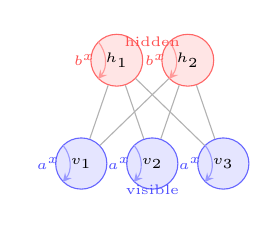
\begin{tikzpicture}[scale=0.82,
        vis/.style={circle,draw=blue!60,fill=blue!10,minimum size=0.65cm,
                    font=\tiny},
        hid/.style={circle,draw=red!60,fill=red!10,minimum size=0.65cm,
                    font=\tiny}]
        \foreach \i/\lbl in {1/$v_1$,2/$v_2$,3/$v_3$}{
          \node[vis] (v\i) at (\i*1.1,0) {\lbl};
          \draw[blue!40,->,>=stealth,bend left=40]
            (v\i.north west) to node[left,font=\tiny,blue!70]{$a^x$}
            (v\i.south west);
        }
        \foreach \j/\lbl in {1/$h_1$,2/$h_2$}{
          \node[hid] (h\j) at (\j*1.1+0.55,1.6) {\lbl};
          \draw[red!40,->,>=stealth,bend left=40]
            (h\j.north west) to node[left,font=\tiny,red!70]{$b^x$}
            (h\j.south west);
        }
        \foreach \i in {1,2,3}
          \foreach \j in {1,2}
            \draw[gray!60,thin] (v\i)--(h\j) node[midway,font=\tiny]{};
        \node[below=0.15cm,font=\tiny,blue!70] at (2.2,0) {visible};
        \node[above=0.05cm,font=\tiny,red!70]  at (2.2,1.6) {hidden};
      \end{tikzpicture}
      \end{center}
      {\small Self-loops denote transverse fields $a_i^x, b_j^x$
       (quantum fluctuations within each unit).}
  \end{columns}
\end{frame}

\begin{frame}{RQBM Gradient and Contrastive Divergence}
  \begin{columns}[T]
    \column{0.52\textwidth}
      For the RQBM, the gradient of the log-likelihood
      w.r.t.\ the inter-layer coupling $W_{ij}$ is:
      \[
        \frac{\partial\ln p(\mathbf{v})}{\partial W_{ij}}
        = \beta\left[
            \langle Z_i^v Z_j^h\rangle_{\rm clamp}
            - \langle Z_i^v Z_j^h\rangle_{\rm free}
          \right]
      \]

      For the transverse-field bias $a_i^x$:
      \[
        \frac{\partial\ln p(\mathbf{v})}{\partial a_i^x}
        = \beta\left[
            \langle X_i^v\rangle_{\rm clamp}
            - \langle X_i^v\rangle_{\rm free}
          \right]
      \]

      \textbf{Key difference from classical:} the quantum gradient
      involves $\langle X_i\rangle$ — an off-diagonal expectation
      value with no classical analogue.
    \column{0.44\textwidth}
      \begin{block}{Quantum CD algorithm}
        \begin{enumerate}
          \item \textbf{Positive phase:}
                clamp $v$ to data; sample $h$ from
                $\rho_h^{(v)} = \Tr_v[\rho_{\rm clamp}]$
          \item \textbf{Negative phase:}
                run $k$ steps of quantum Gibbs
                sampling (Metropolis or QITE) to
                approximate $\rho_{\rm free}$
          \item \textbf{Update:}
                $\Delta W_{ij} \propto
                  \langle Z_iZ_j\rangle_+ -
                  \langle Z_iZ_j\rangle_-$
        \end{enumerate}
      \end{block}
      \begin{alertblock}{Advantage over classical CD}
        Quantum sampling of $\langle X_i\rangle$ and
        $\langle Z_iZ_j\rangle$ is naturally unbiased
        on quantum hardware — no MCMC convergence issue.
      \end{alertblock}
  \end{columns}
\end{frame}

\begin{frame}{RQBM Circuit: Sampling and Inference}
  \textbf{Sampling from the RQBM:} prepare the Gibbs state
  and measure the visible qubits.

  \vspace{0.2cm}
  \begin{center}
  \begin{quantikz}[row sep=0.42cm, column sep=0.4cm]
    \lstick{$\ket{0}_{v_1}$}
      & \gate[5]{V(\phi)} & \meter{} & \cwbend{3} \\
    \lstick{$\ket{0}_{v_2}$}
      & \qw & \meter{} & \cwbend{2} \\
    \lstick{$\ket{0}_{v_3}$}
      & \qw & \meter{} & \cwbend{1} \\
    \lstick{$\ket{0}_{h_1}$}
      & \qw & \qw & \gate[2]{\text{postproc.}} \\
    \lstick{$\ket{0}_{h_2}$}
      & \qw & \qw & \qw
  \end{quantikz}
  \end{center}

  \vspace{0.2cm}
  \begin{columns}[T]
    \column{0.48\textwidth}
      \textbf{Training (positive phase):}
      clamp visible registers to data sample $\mathbf{v}$
      and measure $\langle Z_i^v Z_j^h\rangle$,
      $\langle X_i^v\rangle$, $\langle X_j^h\rangle$.
    \column{0.48\textwidth}
      \textbf{Training (negative phase):}
      run $V(\phi)$ freely; measure the same observables
      to estimate the model expectation values
      $\langle Z_iZ_j\rangle_{\rm free}$.
  \end{columns}
\end{frame}


\begin{frame}{Expressivity of QBMs vs.\ Classical BMs}
  \begin{columns}[T]
    \column{0.52\textwidth}
      \begin{block}{What a classical RBM can represent}
        \begin{itemize}\itemsep0pt
          \item Any distribution over $\{0,1\}^n$
                with sufficiently many hidden units
          \item But: exponentially many hidden units needed
                to replicate some quantum distributions
          \item Limited to diagonal (classical) Hamiltonians
        \end{itemize}
      \end{block}
      \vspace{0.08cm}
      \begin{alertblock}{What a QBM adds}
        \begin{itemize}\itemsep0pt
          \item Off-diagonal elements $\Rightarrow$ coherences
          \item Entangled marginals over visible qubits
          \item Quantum-correlated distributions not realisable
                by any classical latent variable model
        \end{itemize}
      \end{alertblock}
    \column{0.44\textwidth}
      \textbf{Formal expressivity result:}
      Any $n$-qubit $\rho$ is the Gibbs state of some $H$:
      \[
        \rho = \frac{e^{-\beta H}}{Z},\quad
        H = -\beta^{-1}\ln(Z\rho)
      \]
      $\Rightarrow$ QBM is a \emph{universal} model for
      quantum states.
      \vspace{0.1cm}
      \begin{block}{Sample complexity}
        Learning $\rho$ to within $\varepsilon$ requires:
        \[
          N = O\!\left(\frac{n}{\varepsilon^2}\right)
          \text{ samples}
        \]
        (quantum state tomography lower bound).
      \end{block}
  \end{columns}
\end{frame}

\begin{frame}{When Do QBMs Outperform Classical BMs?}
  \begin{columns}[T]
    \column{0.52\textwidth}
      \textbf{Theoretical separation:}
      \begin{enumerate}\small\itemsep1pt
        \item \textbf{Quantum data} (molecular wavefunctions,
              lattice gauge configs): QBM learns directly.
        \item \textbf{Long-range entanglement:}
              exponentially many classical hidden units needed;
              $O(n)$ quantum hidden qubits suffice.
        \item \textbf{Partition function estimation:}
              classical MC suffers sign problems for
              fermionic systems; QBM avoids this.
      \end{enumerate}
      \textbf{Practical regime (NISQ):}
      \begin{itemize}\small\itemsep0pt
        \item Small $n$ ($\lesssim 30$ qubits)
        \item Shallow thermal circuits
        \item Heuristic advantage — not yet provable
      \end{itemize}
    \column{0.44\textwidth}
      \begin{alertblock}{Caution: no-go results}
        For \emph{classical} data distributions:
        \begin{itemize}\small\itemsep1pt
          \item Any QBM can be dequantised if
                quantum correlations of $\rho$ are weak.
          \item Advantage requires genuinely
                quantum off-diagonal structure.
        \end{itemize}
      \end{alertblock}
      \vspace{0.1cm}
      \begin{block}{Barren plateaus in QBMs}
        {\small Like QNNs, deep circuits suffer
        $\mathrm{Var}(\nabla_\theta\mathcal{L})\sim 2^{-n}$.\\
        Mitigation: shallow circuits and
        problem-inspired Hamiltonian structure.}
      \end{block}
  \end{columns}
\end{frame}


\begin{frame}{Outlook: Open Problems and Future Directions}
  \begin{columns}[T]
    \column{0.50\textwidth}
      \begin{block}{Near-term (NISQ) focus}
        \begin{itemize}\small\itemsep0pt
          \item Small QBMs ($n\lesssim 30$) on current hardware
          \item Hybrid: quantum sampling + classical update
          \item Applications: quantum chemistry, finance,
                combinatorial optimisation
          \item Error mitigation for thermal state preparation
        \end{itemize}
      \end{block}
      \vspace{0.05cm}
      \begin{alertblock}{Key open questions}
        \begin{itemize}\small\itemsep0pt
          \item Can QBMs learn classically hard-to-sample
                distributions efficiently?
          \item Can barren plateaus be avoided with
                problem-inspired structure?
          \item Quantum sample complexity advantage?
        \end{itemize}
      \end{alertblock}
    \column{0.46\textwidth}
      \begin{block}{Long-term directions}
        \begin{itemize}\small\itemsep0pt
          \item \textbf{Fault-tolerant QBMs:} exact Gibbs
                state via quantum signal processing
          \item \textbf{Quantum GANs:} replace discriminator
                or generator with a QBM
          \item \textbf{Physics:} learn Hamiltonians from data;
                phase diagrams; sign-problem-free MC
          \item \textbf{Tensor networks:}
                finite-$T$ DMRG $\leftrightarrow$ QBM circuits
        \end{itemize}
      \end{block}
      \vspace{0.05cm}
      {\small\textbf{Quantum advantage landscape:}\\
      $\text{Classical BM}\subset\text{QBM}\subset\text{Full QC}$}
  \end{columns}
\end{frame}

\begin{frame}{Summary: QBM in Context}
  \begin{center}
  \small
  \renewcommand{\arraystretch}{1.05}
  \begin{tabular}{p{2.5cm}p{3.0cm}p{3.0cm}p{3.0cm}}
    \toprule
    & \textbf{Classical BM} & \textbf{QNN} & \textbf{QBM} \\
    \midrule
    State      & $p(\mathbf{v})$      & Pure $\ket{\psi(\theta)}$  & Mixed $\rho(\theta)$ \\
    Model      & $e^{-\beta E}/Z$     & $U(\theta)\ket{0}$         & $e^{-\beta H(\theta)}/Z$ \\
    Gradient   & CD (biased)          & Param-shift                & Thermal avg. \\
    Geometry   & Euclidean            & Fubini-Study QFI           & Bures metric \\
    Training   & Gibbs sampling       & TDVP (real time)           & TDVP (imag.\ time) \\
    Expressiv. & Classical dists.     & Pure states                & All quantum states \\
    Advantage  & Tractable            & Discriminative             & Generative \\
    \bottomrule
  \end{tabular}
  \end{center}
  \vspace{0.05cm}
  \begin{alertblock}{The central message}
    \small
    A QBM is a \textbf{thermal QNN}: it replaces the pure-state ansatz
    with a Gibbs state, enabling generative modelling of quantum
    distributions with a natural connection to statistical mechanics.
  \end{alertblock}
\end{frame}

\begin{frame}{References}
  \begin{columns}[T]
    \column{0.50\textwidth}
      \textbf{Quantum Boltzmann Machines}
      \begin{enumerate}\small\itemsep1pt
        \item M.~H.~Amin et al., \emph{Quantum Boltzmann machine},
              Phys.\ Rev.\ X \textbf{8}, 021050 (2018).
        \item G.~Verdon et al., \emph{A quantum algorithm to train
              neural networks using low-depth circuits},
              arXiv:1712.05304 (2017).
        \item J.~Gao \& L.-M.\ Duan, \emph{Efficient representation
              of quantum many-body states with deep neural networks},
              Nat.\ Commun.\ \textbf{8}, 662 (2017).
        \item C.~Zoufal et al., \emph{Variational quantum Boltzmann
              machines}, Quantum Mach.\ Intell.\ \textbf{3}, 7 (2021).
      \end{enumerate}
    \column{0.46\textwidth}
      \textbf{Thermofield double and Gibbs state preparation}
      \begin{enumerate}\small\itemsep1pt\setcounter{enumi}{4}
        \item S.~Chowdhury et al., \emph{A variational quantum algorithm
              for preparing quantum Gibbs states},
              arXiv:2002.00055 (2020).
        \item D.~Zhu et al., \emph{Generation of thermofield double
              states and critical ground states with a quantum computer},
              PNAS \textbf{117}, 25402 (2020).
      \end{enumerate}
      \textbf{QNN and QFI (see also week15)}
      \begin{enumerate}\small\itemsep1pt\setcounter{enumi}{6}
        \item J.~Stokes et al., \emph{Quantum natural gradient},
              Quantum \textbf{4}, 269 (2020).
        \item M.~H.~Amin, \emph{Searching for quantum speedup in
              quasistatic quantum annealers},
              Phys.\ Rev.\ A \textbf{92}, 052323 (2015).
        \item R.~Babbush et al., \emph{Focus beyond quadratic
              speedups for error-corrected quantum advantage},
              PRX Quantum \textbf{2}, 010103 (2021).
      \end{enumerate}
  \end{columns}
\end{frame}


\section{Summary and perspective for future studies}

% ---- Course philosophy -------------------------------------
\begin{frame}{Course Philosophy and Structure}
  \begin{columns}[T]
    \column{0.55\textwidth}
      \begin{block}{Two main parts}
        \begin{enumerate}
          \item \textbf{Quantum Computing} (Jan--Mar)\\
                Many-body quantum systems, VQE,\\
                fault-tolerant algorithms
          \item \textbf{Quantum Machine Learning} (Apr--May)\\
                NISQ-era variational methods,\\
                QNNs, QPINNs, Boltzmann machines
        \end{enumerate}
      \end{block}
      \vspace{4pt}
      \begin{alertblock}{Central Algorithm}
        The \textbf{Variational Quantum Eigensolver (VQE)}
        links both halves of the course.
      \end{alertblock}
    \column{0.42\textwidth}
      \begin{block}{Key Themes}
        \begin{itemize}
          \item Hilbert spaces \& quantum states
          \item Entanglement \& measurement
          \item Variational circuits (NISQ)
          \item Fault-tolerant algorithms
          \item Quantum-enhanced ML
          \item Solving ODEs/PDEs with quantum methods
        \end{itemize}
      \end{block}
  \end{columns}
\end{frame}

% ---- Week 1 ------------------------------------------------
\begin{frame}{\week{Week 1 (Jan 19--23)} \ Basic Notions of Quantum Mechanics}
  \begin{columns}[T]
    \column{0.48\textwidth}
      \begin{block}{Mathematical Framework}
        \begin{itemize}
          \item Linear algebra reminder
          \item Hilbert spaces and operators
          \item Bra-ket notation: $\ket{\psi}$, $\bra{\phi}$
          \item Inner products \& norms
        \end{itemize}
      \end{block}
    \column{0.48\textwidth}
      \begin{block}{Quantum States}
        \begin{itemize}
          \item One-qubit systems
          \item Pure states vs.\ mixed states
          \item Composite systems
          \item Operator algebra on Hilbert spaces
        \end{itemize}
      \end{block}
  \end{columns}
  \vspace{8pt}
  \begin{alertblock}{Foundation}
    Establish the mathematical language used throughout
    the entire course.
  \end{alertblock}
\end{frame}

% ---- Weeks 2--3 --------------------------------------------
\begin{frame}{\week{Weeks 2--3 (Jan 26 -- Feb 6)} \ Composite Systems, Density Matrices \& Measurements}
  \begin{columns}[T]
    \column{0.48\textwidth}
      \begin{block}{Week 2: Tensor Products \& Entanglement}
        \begin{itemize}
          \item Spectral decomposition
          \item Measurement formalism
          \item Density matrices $\rho = \sum_i p_i \ket{\psi_i}\bra{\psi_i}$
          \item Entanglement: pure \& mixed states
        \end{itemize}
      \end{block}
    \column{0.48\textwidth}
      \begin{block}{Week 3: Density Matrices in Depth}
        \begin{itemize}
          \item Reduced density matrices
          \item Partial traces
          \item Von Neumann entropy
          \item Entanglement measures
        \end{itemize}
      \end{block}
  \end{columns}
  \vspace{6pt}
  \begin{block}{Key Concept: Entanglement}
    \[
      \ket{\Phi^+} = \frac{1}{\sqrt{2}}\bigl(\ket{00}+\ket{11}\bigr)
      \quad\Rightarrow\quad S(\rho_A) = \log 2
    \]
  \end{block}
\end{frame}

% ---- Week 4 ------------------------------------------------
\begin{frame}{\week{Week 4 (Feb 9--13)} \ Entanglement, Entropies \& Quantum Gates}
  \begin{columns}[T]
    \column{0.48\textwidth}
      \begin{block}{Entanglement \& Entropies}
        \begin{itemize}
          \item Review of density matrices
          \item Entanglement entropies
          \item Separability criteria
        \end{itemize}
      \end{block}
    \column{0.48\textwidth}
      \begin{block}{Quantum Gates (Introduction)}
        \begin{itemize}
          \item Single-qubit gates: $X$, $Y$, $Z$, $H$, $S$, $T$
          \item Two-qubit gates: CNOT, CZ, SWAP
          \item Gate universality
          \item Simple Hamiltonian systems
        \end{itemize}
      \end{block}
  \end{columns}
  \vspace{6pt}
  \begin{alertblock}{Bridge to VQE}
    Understanding gates and Hamiltonians prepares for the VQE algorithm.
  \end{alertblock}
\end{frame}

% ---- Week 5 ------------------------------------------------
\begin{frame}{\week{Week 5 (Feb 16--20)} \ Getting Started with the VQE Algorithm}
  \begin{columns}[T]
    \column{0.55\textwidth}
      \begin{block}{Quantum Gates \& Simple Algorithms}
        \begin{itemize}
          \item Quantum circuit model
          \item Parameterised circuits (ansätze)
          \item Gate decompositions
          \item One- \& two-qubit Hamiltonians
        \end{itemize}
      \end{block}
      \vspace{4pt}
      \begin{block}{VQE Overview}
        \[
          E(\bm{\theta}) = \bra{\psi(\bm{\theta})}H\ket{\psi(\bm{\theta})}
          \;\geq\; E_0
        \]
        Minimise $E(\bm\theta)$ over circuit parameters $\bm\theta$.
      \end{block}
    \column{0.42\textwidth}
      \begin{alertblock}{Project 1}
        Implement VQE for simple\\
        one- and two-qubit Hamiltonians.\\[4pt]
        \textbf{Key tasks:}
        \begin{itemize}
          \item Design ansatz circuit
          \item Evaluate energy expectation
          \item Classical optimisation loop
        \end{itemize}
      \end{alertblock}
  \end{columns}
\end{frame}

% ---- Week 6 ------------------------------------------------
\begin{frame}{\week{Week 6 (Feb 23--27)} \ Implementing VQE: Measurements \& Gradients}
  \begin{columns}[T]
    \column{0.55\textwidth}
      \begin{block}{Advanced VQE Topics}
        \begin{itemize}
          \item \textbf{Parameter-shift rule} for gradients:
                \[
                  \partial_\theta E = \tfrac{E(\theta+\frac\pi2)-E(\theta-\frac\pi2)}{2}
                \]
          \item Adaptive VQE (ADAPT-VQE)
          \item Shot-noise and measurement strategies
          \item Simulation codes and debugging
        \end{itemize}
      \end{block}
    \column{0.42\textwidth}
      \begin{block}{Hamiltonians Explored}
        \begin{itemize}
          \item One-qubit spin models
          \item Two-qubit interacting systems
          \item Mapping physics to qubits
          \item Introduction to the\\
                \textbf{Lipkin model}
        \end{itemize}
      \end{block}
  \end{columns}
\end{frame}

% ---- Weeks 7--8 --------------------------------------------
\begin{frame}{\week{Weeks 7--8 (Mar 2--13)} \ VQE for the Lipkin Model \& Jordan-Wigner}
  \begin{columns}[T]
    \column{0.48\textwidth}
      \begin{block}{Week 7: Lipkin Model VQE}
        \begin{itemize}
          \item Two-qubit Hamiltonian implementation
          \item Full VQE pipeline for the\\
                Lipkin collective model
          \item Benchmarking against exact diagonalisation
          \item Circuit optimisation strategies
        \end{itemize}
      \end{block}
    \column{0.48\textwidth}
      \begin{block}{Week 8: Fermionic Hamiltonians}
        \begin{itemize}
          \item Lipkin model: final results
          \item \textbf{Jordan-Wigner transformation}:
                \[
                  a_j \;\rightarrow\; Z^{\otimes j}\otimes\sigma^-
                \]
          \item Mapping fermionic operators to qubits
          \item Beyond the Lipkin model
        \end{itemize}
      \end{block}
  \end{columns}
  \vspace{4pt}
  \begin{alertblock}{Milestone}
    Project 1 results in a working VQE solver.
  \end{alertblock}
\end{frame}

% ---- Week 9 ------------------------------------------------
\begin{frame}{\week{Week 9 (Mar 16--20)} \ Quantum Fourier Transforms}
  \begin{columns}[T]
    \column{0.55\textwidth}
      \begin{block}{From NISQ to Fault-Tolerant Algorithms}
        \begin{itemize}
          \item Discrete Fourier Transform review
          \item \textbf{Quantum Fourier Transform (QFT)}:
                \[
                  \mathrm{QFT}\ket{j} = \frac{1}{\sqrt{N}}
                  \sum_{k=0}^{N-1} e^{2\pi i jk/N}\ket{k}
                \]
          \item Circuit decomposition: $O(n^2)$ gates vs.\ $O(n\,2^n)$
        \end{itemize}
      \end{block}
    \column{0.42\textwidth}
      \begin{block}{QFT Circuit Structure}
        \begin{itemize}
          \item Hadamard gates
          \item Controlled phase rotations $R_k$
          \item Bit-reversal permutation
          \item Exponential speedup over classical FFT
        \end{itemize}
      \end{block}
  \end{columns}
\end{frame}

% ---- Weeks 10--11 ------------------------------------------
\begin{frame}{\week{Weeks 10--11 (Mar 23 -- Apr 10)} \ QFT, Quantum Phase Estimation \& HHL}
  \begin{columns}[T]
    \column{0.48\textwidth}
      \begin{block}{Quantum Phase Estimation (QPE)}
        \begin{itemize}
          \item QFT as subroutine
          \item Estimating eigenvalues of $U$:
                \[
                  U\ket{u} = e^{2\pi i\varphi}\ket{u}
                \]
          \item Circuit construction \& precision
          \item Applications to chemistry \& physics
        \end{itemize}
      \end{block}
    \column{0.48\textwidth}
      \begin{block}{HHL Algorithm (Linear Systems)}
        \begin{itemize}
          \item Solving $A\bm{x}=\bm{b}$ on a quantum computer
          \item Uses QPE as subroutine
          \item Exponential speedup (sparse, well-conditioned $A$)
          \item Implementation and codes
          \item Limitations and caveats
        \end{itemize}
      \end{block}
  \end{columns}
\end{frame}

% ---- Week 12 -----------------------------------------------
\begin{frame}{\week{Week 12 (Apr 13--17)} \ HHL Algorithm: Codes \& Implementation}
  \begin{columns}[T]
    \column{0.55\textwidth}
      \begin{block}{Deep Dive into HHL}
        \begin{itemize}
          \item Full circuit implementation
          \item Ancilla qubit rotation: eigenvalue inversion
          \item Amplitude encoding of $\bm{b}$
          \item Uncomputation and measurement
          \item Error analysis and success probability
        \end{itemize}
      \end{block}
    \column{0.42\textwidth}
      \begin{alertblock}{HHL Complexity}
        \[
          \mathcal{O}\!\left(\log N \cdot \kappa^2 \cdot \frac{1}{\epsilon}\right)
        \]
        vs.\ classical $\mathcal{O}(N^3)$\\[4pt]
        where $\kappa$ = condition number,\\
        $\epsilon$ = precision,\\
        $N$ = matrix dimension.
      \end{alertblock}
    \end{columns}
    \vspace{4pt}
    \begin{block}{Transition to Quantum Machine Learning}
      With QFT, QPE and HHL covered, we now turn to the
      \textbf{NISQ-era QML} methods for the remainder of the course.
    \end{block}
\end{frame}

% ---- Week 13 -----------------------------------------------
\begin{frame}{\week{Week 13 (Apr 20--24)} \ QAOA: Quantum Approximate Optimisation}
  \begin{columns}[T]
    \column{0.55\textwidth}
      \begin{block}{QAOA Algorithm}
        \begin{itemize}
          \item Combinatorial optimisation problems
          \item Alternating cost and mixer unitaries:
                \[
                  \ket{\bm\gamma,\bm\beta}
                  = U_M(\beta_p)\,U_C(\gamma_p)\cdots
                    U_M(\beta_1)\,U_C(\gamma_1)\ket{+}^{\otimes n}
                \]
          \item Classical outer-loop optimisation
          \item Depth-$p$ approximation ratio
        \end{itemize}
      \end{block}
    \column{0.42\textwidth}
      \begin{block}{Implementation Focus}
        \begin{itemize}
          \item Mapping problems to Ising Hamiltonians
          \item Circuit construction
          \item Gradient evaluation
          \item Benchmarking on toy instances
        \end{itemize}
      \end{block}
  \end{columns}
  \vspace{4pt}
  \begin{alertblock}{Connection}
    QAOA is the optimisation counterpart to VQE and serves as
    a gateway into Quantum Machine Learning methods.
  \end{alertblock}
\end{frame}

% ---- Week 14 -----------------------------------------------
\begin{frame}{\week{Week 14 (Apr 27 -- May 1)} \ Quantum Machine Learning: Foundations}
  \begin{columns}[T]
    \column{0.55\textwidth}
      \begin{block}{QML Basics}
        \begin{itemize}
          \item What is QML? Taxonomy of approaches
          \item Data encoding strategies:\\
                amplitude, angle, IQP, etc.
          \item Parameterised quantum circuits as models
          \item Expressibility and entangling capacity
          \item Barren plateaus and trainability
        \end{itemize}
      \end{block}
    \column{0.42\textwidth}
      \begin{block}{Quantum Neural Networks}
        \begin{itemize}
          \item QNN architecture overview
          \item Layered variational circuits
          \item Loss functions \& gradients
          \item Links to classical deep learning
          \item Connections to QAOA
        \end{itemize}
      \end{block}
  \end{columns}
\end{frame}

% ---- Weeks 15--16 ------------------------------------------
\begin{frame}{\week{Weeks 15--16 (May 4--15)} \ QPINNs: Solving Differential Equations}
  \begin{columns}[T]
    \column{0.48\textwidth}
      \begin{block}{Physics-Informed QNNs}
        \begin{itemize}
          \item Classical PINNs review
          \item \textbf{Quantum PINNs (QPINNs)}:
                replace neural network with\\
                a parameterised quantum circuit
          \item Encoding PDEs as loss functions
          \item Automatic differentiation on circuits
        \end{itemize}
      \end{block}
    \column{0.48\textwidth}
      \begin{block}{Applications \& Implementation}
        \begin{itemize}
          \item Solving ODEs and PDEs:\\
                Schrödinger, heat, Poisson
          \item Boundary condition encoding
          \item Gradient computation via\\
                parameter-shift rule
          \item Discussion of codes
        \end{itemize}
      \end{block}
  \end{columns}
  \vspace{4pt}
  \begin{alertblock}{Key Idea}
    QPINNs marry the physics-informed training paradigm with
    the expressive power of quantum circuits to solve differential
    equations on near-term hardware.
  \end{alertblock}
\end{frame}

% ---- Week 17 -----------------------------------------------
\begin{frame}{\week{Week 17 (May 18--22)} \ Quantum Boltzmann Machines}
  \begin{columns}[T]
    \column{0.55\textwidth}
      \begin{block}{Quantum Boltzmann Machines (QBM)}
        \begin{itemize}
          \item Classical RBM / BM recap
          \item Quantum generalisation:\\
                thermal states as model distributions
          \item Training via quantum log-likelihood gradients
          \item Transverse-field Hamiltonians as model parameters
          \item Restricted QBM (RQBM) architecture
        \end{itemize}
      \end{block}
    \column{0.42\textwidth}
      \begin{block}{Connections \& Outlook}
        \begin{itemize}
          \item Links to VQE and variational circuits
          \item Generative quantum models
          \item Applications in physics \& optimisation
          \item Open research problems
        \end{itemize}
      \end{block}
  \end{columns}
  \vspace{4pt}
  \begin{alertblock}{Course Conclusion}
    QBMs illustrate how quantum statistical mechanics and
    machine learning merge
  \end{alertblock}
\end{frame}

% ---- Course map: Part 1 ------------------------------------
\begin{frame}{Course Road Map --- Part 1: Quantum Computing}
  \begin{center}
  \small
  \renewcommand{\arraystretch}{1.28}
  \begin{tabular}{@{}llp{8.0cm}@{}}
    \toprule
    \textbf{Weeks} & \textbf{Dates} & \textbf{Topics} \\
    \midrule
    1     & Jan 19--23     & Basic quantum mechanics, Hilbert spaces, qubits \\
    2--3  & Jan 26--Feb 6  & Composite systems, density matrices, entanglement \\
    4     & Feb 9--13      & Entanglement entropies, quantum gates \\
    5--6  & Feb 16--27     & VQE: algorithm, measurements, gradients (Project 1) \\
    7--8  & Mar 2--13      & VQE for Lipkin model, Jordan-Wigner transform \\
    9     & Mar 16--20     & Quantum Fourier Transform \\
    10--11& Mar 23--Apr 10 & QPE and HHL algorithm \\
    12    & Apr 13--17     & HHL codes and implementation \\
    \bottomrule
  \end{tabular}
  \end{center}
\end{frame}

% ---- Course map: Part 2 ------------------------------------
\begin{frame}{Course Road Map --- Part 2: Quantum Machine Learning}
  \begin{center}
  \small
  \renewcommand{\arraystretch}{1.28}
  \begin{tabular}{@{}llp{8.0cm}@{}}
    \toprule
    \textbf{Weeks} & \textbf{Dates} & \textbf{Topics} \\
    \midrule
    13    & Apr 20--24     & QAOA: quantum approximate optimisation \\
    14    & Apr 27--May 1  & QML foundations, Quantum Neural Networks \\
    15--16& May 4--15      & QPINNs: solving differential equations \\
    17    & May 18--22     & Quantum Boltzmann Machines and course summary \\
    \bottomrule
  \end{tabular}
  \end{center}
  \vspace{6pt}
  \begin{alertblock}{Overarching Goal}
    Equip participants with the theoretical foundations and practical
    implementation skills to design, analyse, and run quantum algorithms
    on near-term and fault-tolerant hardware.
  \end{alertblock}
\end{frame}

% ---- Closing -----------------------------------------------
\begin{frame}{Summary: What we have done}
  \begin{columns}[T]
    \column{0.48\textwidth}
      \begin{block}{Part 1 -- Quantum Computing}
        \begin{itemize}
          \item Formalism of quantum mechanics
          \item Entanglement \& density matrices
          \item Variational algorithms (VQE)
          \item Fault-tolerant algorithms:\\
                QFT, QPE, HHL
          \item Physical models: Lipkin, Pairing
        \end{itemize}
      \end{block}
    \column{0.48\textwidth}
      \begin{block}{Part 2 -- Quantum ML}
        \begin{itemize}
          \item QAOA for optimisation
          \item Quantum Neural Networks
          \item Physics-Informed QNNs\\
                (QPINNs)
          \item Quantum Boltzmann Machines
          \item Connections to classical ML
        \end{itemize}
      \end{block}
  \end{columns}
  \vspace{8pt}
  \begin{alertblock}{Overarching Goal}
    Equip course participants with the theoretical foundations
    and practical implementation skills to design, analyse, and run
    quantum algorithms on near-term and fault-tolerant hardware.
  \end{alertblock}
\end{frame}

% ============================================================
%  PERSPECTIVES — QUANTUM COMPUTING: FUTURE DIRECTIONS
% ============================================================

% ---- Perspectives: section divider -------------------------
\begin{frame}[plain]
  \begin{center}
    \vspace{1.4cm}
    {\Huge\bfseries\color{qblue} Perspectives}\\[0.5em]
    {\Large\color{black} Future Directions in Quantum Computing}\\[0.3em]
    {\normalsize\color{gray} Algorithms, Hardware, and Scientific Applications}
  \end{center}
\end{frame}

% ---- Perspectives 1: NISQ & fault-tolerant algorithms ------
\begin{frame}{Perspectives --- Algorithms: NISQ and Fault-Tolerant}
  \begin{columns}[T]
    \column{0.48\textwidth}
      \begin{block}{Near-Term (NISQ) Algorithms}
        \begin{itemize}\footnotesize\itemsep1pt
          \item \textbf{Improved VQE ans\"{a}tze:}
                hardware-efficient, UCC, ADAPT-VQE,
                symmetry-preserving circuits
          \item \textbf{Quantum error mitigation:}
                zero-noise extrapolation,
                probabilistic error cancellation
          \item \textbf{Barren plateau remedies:}
                layerwise training, local cost
                functions, better initialisation
          \item \textbf{Advantage benchmarks:}
                tasks where NISQ devices
                outperform classical methods
        \end{itemize}
      \end{block}
    \column{0.48\textwidth}
      \begin{block}{Fault-Tolerant Algorithms}
        \begin{itemize}\footnotesize\itemsep1pt
          \item \textbf{Quantum simulation:}
                Trotterisation, qubitisation,
                linear combination of unitaries (LCU)
          \item \textbf{Improved QPE:}
                randomised and Bayesian phase
                estimation with fewer qubits
          \item \textbf{Beyond HHL:}
                quantum linear algebra (QSVM,
                quantum PCA), dequantisation
          \item \textbf{Quantum walks \& search:}
                Grover speedups, walk-based
                graph algorithms, Monte Carlo
        \end{itemize}
      \end{block}
  \end{columns}
\end{frame}

% ---- Perspectives 2: Physical sciences applications --------
\begin{frame}{Perspectives --- Applications in the Physical Sciences}
  \begin{columns}[T]
    \column{0.48\textwidth}
      \begin{block}{Quantum Chemistry and Nuclear Physics}
        \begin{itemize}\footnotesize\itemsep1pt
          \item \textbf{Electronic structure:}
                VQE and QPE for ground and excited
                states beyond coupled-cluster reach
          \item \textbf{Nuclear structure:}
                ab initio calculations using Lipkin,
                pairing, and shell-model Hamiltonians
          \item \textbf{Quantum advantage:}
                fault-tolerant simulation of strongly
                correlated systems (e.g.\ FeMoco)
          \item \textbf{Imaginary-time evolution:}
                thermal states and finite-temperature
                properties on quantum hardware
        \end{itemize}
      \end{block}
    \column{0.48\textwidth}
      \begin{block}{Condensed Matter and High-Energy Physics}
        \begin{itemize}\footnotesize\itemsep1pt
          \item \textbf{Lattice gauge theories:}
                quantum simulation of QED, QCD,
                and the Hubbard model
          \item \textbf{Topological phases:}
                preparation and detection of
                topological order and anyons
          \item \textbf{Quantum gravity:}
                holographic duality (AdS/CFT)
                encoded on quantum circuits
          \item \textbf{Quantum sensing:}
                Heisenberg-limited parameter
                estimation, magnetometry,
                gravimetry
        \end{itemize}
      \end{block}
  \end{columns}
\end{frame}

% ---- Perspectives 3: QML, hardware, open challenges --------
\begin{frame}{Perspectives --- Quantum ML, Hardware, and Open Challenges}
  \begin{columns}[T]
    \column{0.54\textwidth}
      \begin{block}{Quantum Machine Learning Frontiers}
        \begin{itemize}\footnotesize\itemsep1pt
          \item \textbf{Quantum generative models:}
                quantum GANs, quantum diffusion,
                and QBMs beyond the RQBM
          \item \textbf{Quantum reinforcement learning:}
                RL on quantum hardware for
                quantum control and agentic workflows
          \item \textbf{Classical--quantum hybrid:}
                tensor networks and classical
                circuit simulation as a guide
          \item \textbf{Certification:}
                classical shadow tomography
                and cross-entropy benchmarking
        \end{itemize}
      \end{block}
    \column{0.43\textwidth}
      \begin{block}{Hardware and Open Challenges}
        \begin{itemize}\footnotesize\itemsep1pt
          \item \textbf{Qubit platforms:}
                superconducting, trapped-ion,
                photonic, neutral-atom arrays
          \item \textbf{Error correction:}
                surface and color codes;
                logical fault-tolerant qubits
          \item \textbf{Scalability:}
                how many logical qubits for
                quantum advantage on
                real-world problems?
        \end{itemize}
      \end{block}
      \begin{alertblock}{Key Insight}
        {\small Quantum advantage requires both
        better algorithms \emph{and}
        better hardware in tandem.}
      \end{alertblock}
  \end{columns}
\end{frame}

\end{document}
